\documentclass[11pt,a4paper]{article}
\ifdefined\pdfminorversion\pdfminorversion=7\fi
\usepackage[T1]{fontenc}
\usepackage[utf8]{inputenc}
\usepackage{lmodern}
\usepackage[a4paper,margin=25mm,headheight=14pt]{geometry}
\usepackage{amsmath,amssymb}
\usepackage{booktabs}
\usepackage{enumitem}
\usepackage{microtype}
\usepackage{tabularx}
\usepackage{xcolor}
\usepackage{pid-rs-report-tables}
\usepackage{float}
\usepackage[unicode]{hyperref}
\usepackage{xurl}
\usepackage{fancyhdr}
\usepackage{graphicx}
\usepackage{needspace}

\newcolumntype{L}[1]{>{\raggedright\arraybackslash}p{#1}}
\newcolumntype{Y}{>{\raggedright\arraybackslash}X}
\setlength{\emergencystretch}{3em}

\ifdefined\pdfinfoomitdate\pdfinfoomitdate=1\fi
\ifdefined\pdftrailerid\pdftrailerid{}\fi
\ifdefined\pdfsuppressptexinfo\pdfsuppressptexinfo=15\fi
\hypersetup{%
  hidelinks,
  pdftitle={KSG revision-4 M1a composite-v5 successor boundary},
  pdfauthor={Sepehr Mahmoudian},
  pdfsubject={Append-only hosted-qualification failure and successor contract},
  pdfkeywords={KSG, evidence custody, hosted qualification, append-only repair, PID boundaries}
}

\newcommand{\Status}[1]{\textsf{#1}}
\newcommand{\Contract}[1]{\ensuremath{\mathsf{#1}}}
\newcommand{\Important}[1]{\textcolor{PidPrimary}{\textbf{#1}}}

\PidConfigureSections
\PidSetRunningHeads{pid-rs composite-v5}{KSG hosted-qualification boundary}
\PidConfigureAbstract
\PidConfigureLinksAndListings

\setlength{\parindent}{0pt}
\setlength{\parskip}{5pt}
\setlist{nosep,leftmargin=5mm}
\renewcommand{\arraystretch}{1.17}

\title{\PidReportTitle
  {KSG Revision-4 M1a Composite-v5 Successor Boundary}
  {Why a published failed attempt cannot issue a receipt}}
\author{pid-rs project analysis}
\date{18 August 2026}

\begin{document}
\PidMakeTitle

\begin{abstract}
Published commit
\path{da253576a5f76e99633fff4de5cf1118f967b90d} is the exact composite-v4 C4
subject. Its local closure passed, but its first hosted qualification did not: CodeQL passed,
repository CI contained three terminal job failures, and the dedicated v4 route failed at the
static-validation preflight before substantive contract validation completed. This report records
why R4 is permanently unissued, defines an append-only C5
successor with four bounded repairs and a fresh Lean replay, and permits R5 only after fresh
attempt-1 success of every required route. It changes no theorem, estimator, PID object, or
numerical result.
\end{abstract}

\begin{center}
\fcolorbox{PidAccent}{PidSoft}{\parbox{0.92\linewidth}{%
\Important{Disposition.} C4 remains an immutable published subject. Its failure is retained as
process evidence, not converted into partial qualification. R4 is unissued. C5 and any later R5
are new commits with new evidence. This report is not a KSG proof, PID validation, authentication,
attestation, independence finding, peer review, or application gate.
}}
\end{center}

\section{Decision from first principles}

For exact C4, define
\begin{equation}
  Q_4 = \mathrm{CI}_4 \land \mathrm{CodeQL}_4 \land D_4,
  \label{eq:q4}
\end{equation}
where each term means terminal success at run attempt 1 for the same exact C4 commit, and
\(D_4\) is the dedicated composite-v4 route. The observations are
\begin{equation}
  \mathrm{CI}_4=\mathrm{false},\qquad
  \mathrm{CodeQL}_4=\mathrm{true},\qquad
  D_4=\mathrm{false}.
  \label{eq:q4-values}
\end{equation}
Substitution of Equation~(2) into Equation~(1) gives \(Q_4=\mathrm{false}\). The frozen
issuance rule is
\begin{equation}
  \operatorname{issue}(R4) \Longleftrightarrow Q_4.
  \label{eq:r4}
\end{equation}
Therefore R4 is permanently unissued. A passing CodeQL term cannot compensate for either failed
term. A rerun would use \texttt{run\_attempt = 2}; rewriting C4 would replace the published
subject. Neither operation can satisfy the attempt-1 rule.

\section{Exact hosted observations}

\begin{table}[H]
\centering
\small
\begin{tabularx}{\linewidth}{@{}L{0.23\linewidth}L{0.21\linewidth}Y@{}}
\toprule
\PidTableHeaderRow
\textbf{Route} & \textbf{Run / result} & \textbf{Bounded interpretation} \\
\midrule
Repository CI & \texttt{32079866560}; failed & Three terminal job failures; the all-jobs-success term is false. \\
CodeQL & \texttt{32079865482}; passed & Actions, JavaScript/TypeScript, Python, and Rust passed; only the CodeQL term is true. \\
Dedicated v4 & \texttt{32079866461}; failed & Checkout residue was rejected at the static-validation preflight; substantive validation did not complete. \\
Dependency Graph & \texttt{32079867694}; passed & Context only; neither a term in \(Q_4\) nor a captured qualification role. \\
\bottomrule
\end{tabularx}
\caption{C4 hosted observations. Route labels do not make the provider authoritative or transfer
credit among routes.}
\label{tab:c4-hosted}
\end{table}

The predecessor capture is retained in C5 as no-credit failure evidence. Provider responses and
artifact archives are bounded observations. They do not authenticate GitHub, prove a complete
provider history, or establish scientific validity.

\section{Four bounded repairs}

\begin{table}[H]
\centering
\small
\begin{tabularx}{\linewidth}{@{}L{0.18\linewidth}L{0.22\linewidth}Y@{}}
\toprule
\PidTableHeaderRow
\textbf{Surface} & \textbf{Epistemic status} & \textbf{C5 repair and retained boundary} \\
\midrule
Checkout residue & Exact causal reproduction & Accept absence or the one reviewed 83-byte regular, single-link image; verify SHA-256; unlink the literal entry; require absence. Every other object or byte image rejects. \\
Release fixture & Root cause not uniquely established by the log & Stop moving the live fixture's \texttt{.git}; use distinct archive fixtures, phase diagnostics, and a hostile ancestor repository. Require fresh hosted requalification. \\
Zeta firewall & Exact reviewed byte drift & Preserve \texttt{uncertified}; rebind the 37,869-byte section at SHA-256 \texttt{d1a1775d\ldots d4d368}; retain the unrelated-section negative control. \\
Certified SxPID & Exact stale current bindings & Rebind the final release dependency, execution-container, documentation, and support-gate bytes; retain a membership-preserving exact-line mutation. \\
\bottomrule
\end{tabularx}
\caption{A local repair is necessary, not sufficient. The release-fixture row deliberately does
not claim a causal diagnosis that the retained hosted log cannot establish.}
\label{tab:repairs}
\end{table}

The checkout normalizer never implements a general \texttt{rm}. The accepted residue SHA-256 is
\path{443a5f645c23c3d0c0aa09f634b2ad111d46ef61946b598a2fb311678ab47454}.
Symlinks, directories, hard links, altered bytes, altered permissions, and route changes fail
closed.

The zeta rebind changes spelling custody only. The certified-SxPID rebind does not turn a finite
exact certifier into a population theorem, a Rust refinement proof, or a general validation of
shared-exclusions PID.

\Needspace{10\baselineskip}
\section{Append-only C5 and R5 topology}

C5 is the exact unsigned direct child of C4, with message
\texttt{Repair KSG M1a composite v5 contract}. R5, if permitted, is the exact unsigned direct
child of C5, with message \texttt{Record KSG M1a composite v5 receipt}. No v4 capture or receipt
path is reused.

Define
\begin{equation}
  Q_5 = L_5 \land \mathrm{CI}_5 \land \mathrm{CodeQL}_5 \land D_5,
  \label{eq:q5}
\end{equation}
where \(L_5\) is local static, hostile, replay, source-state, and publication closure;
\(\mathrm{CI}_5\) is repository-CI all-jobs success; \(\mathrm{CodeQL}_5\) is success of every
required CodeQL role; and \(D_5\) is success of the dedicated composite-v5 workflow. Every term
must be terminal at attempt 1 for the same exact C5 commit. The new issuance rule is
\begin{equation}
  \operatorname{issue}(R5) \Longleftrightarrow Q_5.
  \label{eq:r5}
\end{equation}
Any false, missing, nonterminal, wrong-commit, or wrong-attempt term leaves R5 unissued and requires
another append-only contract version.

\begin{figure}[H]
\centering
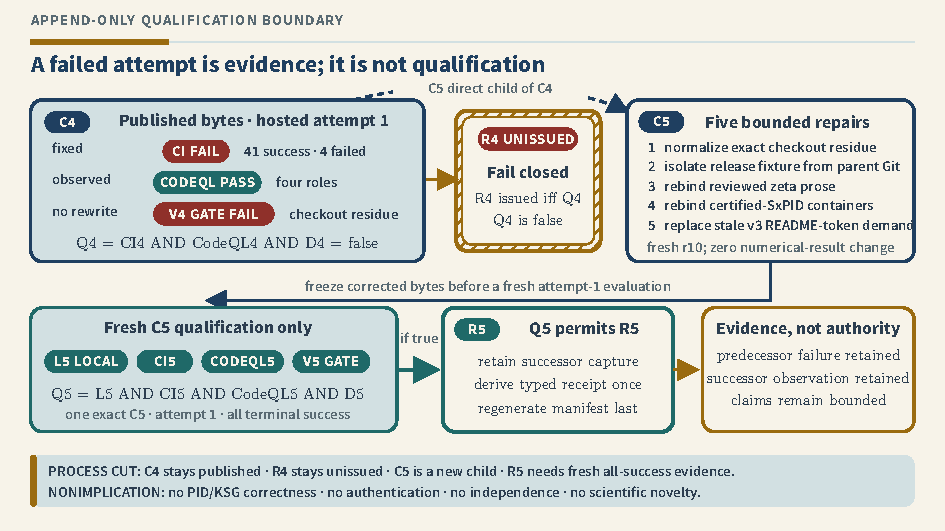
\includegraphics[
  width=\linewidth,
  alt={C4 is published but its CI and dedicated v4 routes failed, so Q4 is false and R4 is unissued. A direct-child C5 makes four bounded repairs. Only fresh attempt-1 local, CI, CodeQL, and dedicated-v5 success can make Q5 true and permit R5, whose evidence remains process custody rather than scientific authority.}
]{figures/ksg-m1a-composite-v5-boundary/c4-failure-c5-r5.pdf}
\caption{Append-only qualification boundary. The diagram distinguishes a retained failed attempt,
a new repair commit, and a new all-success receipt route. It does not encode scientific transfer or
authority.}
\label{fig:v5-boundary}
\end{figure}

When \(Q_5\) is true, R5 changes exactly three paths: it adds the raw successor capture, adds the
typed receipt derived from that capture, and regenerates the self-excluding current-source manifest
last. The receipt hashes both the predecessor-failure capture retained in C5 and the
successor-qualification capture added in R5. The manifest inventories both R5 additions while
excluding itself. R5's tree and commit are outputs, never checksum inputs.

\section{Replay, durability, and publication scope}

C5 publishes a fresh Lean 4.33 replay as \texttt{r10}; accepted C4 \texttt{r9} remains
exact-hash-bound prior execution evidence. The suffix is numbering metadata: the tenth receipt in the
12-August sequence and the eleventh current-project replay overall because the separate 11-August
historical receipt is outside that sequence. It is not a theorem revision, proof-strength rank, or
independence claim.

Remote \texttt{main} is a minimum operational recovery anchor only under provider-retention and
history-rewrite assumptions. The recovery record must identify the remote URL, ref, commit OID,
tree OID, parent OID, and push observation. Remote \texttt{main} is mutable, not a scholarly
archive. A publication freeze should also retain the exact commit and its load-bearing predecessor
and successor captures, typed receipt, replay receipt, path policy, source manifest, report and
visual-review sources, figure source, and rendered PDF in a versioned release or recognized
content-addressed archive, with access, licence, retention, and retrieval checks. A digest without
a retrievable preimage receives commitment or bounded-omission credit only.

No branch, worktree, or temporary directory is deleted until exact-byte or semantic supersession is
proved and every unique permitted payload has a remote or otherwise independent durable home.

\Needspace{12\baselineskip}
\section{Review lenses and nonclaims}

The boundary is reviewed separately for logical implication, Git topology, hosted semantics,
schema closure, adversarial causality, Python isolation, shell failure handling, Lean custody, PDF
objects, raster layout, SVG accessibility, numerical scope, method provenance, PID-family
separation, security, privacy, durability, reproducibility, usability, and publication English.
Disagreement remains visible until adjudicated; a digest alone does not preserve dissent.

A separate correlated agent red-team found and corrected the original topology, run-status
language, permission claim, incomplete \(Q_5\) definitions, dual-capture binding, and durability
omissions. This records review provenance but grants no dependency-disjoint, independent, or
human-review credit.

This process can prevent known classes of evidence error. It does not demonstrate a causal
improvement in research quality, replace peer review, or make the process itself publishable.
Methods-report eligibility is necessary, not sufficient, and requires disclosure of attempt
population, adaptive exposures, stopping and selection, deviations, failures, inconclusive results,
resources and AI roles, dissent, human adjudication, materials, access, and licences.

Composite-v5 adds zero PID theories, zero PID functionals, zero estimators, zero theorem-source
changes, and zero numerical-result changes. Nothing here transfers evidence among categorical MGW,
Schick--Poland, Ehrlich continuous shared exclusions, KSG mutual information, Williams--Beer
\(I_{\min}\), PID2, PID3, quantized, or mixed-support routes. Nothing here establishes
authentication, attestation, authorship, independence, peer review, provider completeness,
application fitness, control authority, or evidence for a drone or other ecosystem deployment.

\end{document}
